\chapter{Arcane stuff}

% pointer haha hehe

% this chapter for stuff which are too far from py to actually have a comparison

This chapter sheds light onto concepts that are too dissimilar to Python to actually have a comparison.
For the most part, these concepts especially involving \textit{pointers} can be difficult to understand at first.
However, it is still possible to be able to grasp these concepts given ample time and practice.
Since this guide is meant to be a quick guide, we will not dabble too deep into the following concepts unless necessary to alleviate as many gray areas as possible.

\textit{Brace yourselves, you're in for quite a ride.}

\section{What is a pointer?}

A \textbf{pointer variable} (simply referred as a \textit{pointer}) stores memory address values where another value is located.
Pointers are declared by adding a dereferencing operator (i.e., an asterisk, \verb|*|) either before a given name (e.g., \verb|*ptr|), or after the data type (e.g., \verb|int*|).
For consistency, the asterisk will be placed just before the pointer variable's name.

\begin{minted}{c}
/* Declaring an int pointer variable */
int *ptr1; // we will use this convention
int* ptr2; // also valid, but not used here
\end{minted}

The main difference between a typical variable and a pointer is that a variable directly references a value, whilst a pointer indirectly references a value.
To help illustrate this, refer to the following code and the corresponding output (denoted in comments).

\begin{minted}[linenos]{c}
// Declare a pointer variable named ptr
int *ptr;

// Set ptr to point to a different memory address containing the value 1
*ptr = 1;

printf("%d\n", *ptr); // 1
printf("%p\n", ptr);  // 0x7ff7b77f61c0
printf("%p\n", &ptr); // 0x7ff7b77f6180
\end{minted}

Note that printing the value of \verb|*ptr| and \verb|ptr| render different results.
Also, if the code is compiled and run a second time, the address value produced from printing the value of \verb|ptr| may change.
Here, \verb|ptr| directly references (contains) a memory address value, which is the location where that value of 1 is stored in memory.
This memory address value uses the \verb|%p| conversion specifier.

It can also be implied from here that variables occupy an address in memory, and this includes pointers as well.
We can view the address of any variable using the address operator (i.e., ampersand, \verb|&|).
Continuing from the previous example, printing the value of \verb|&ptr| produces the memory address where the pointer \verb|ptr| is located.
Compiling and running the code a second time may also once again change the printed address value.

\begin{minted}{c}
printf("%p\n", &ptr);
\end{minted}

\begin{figure}
    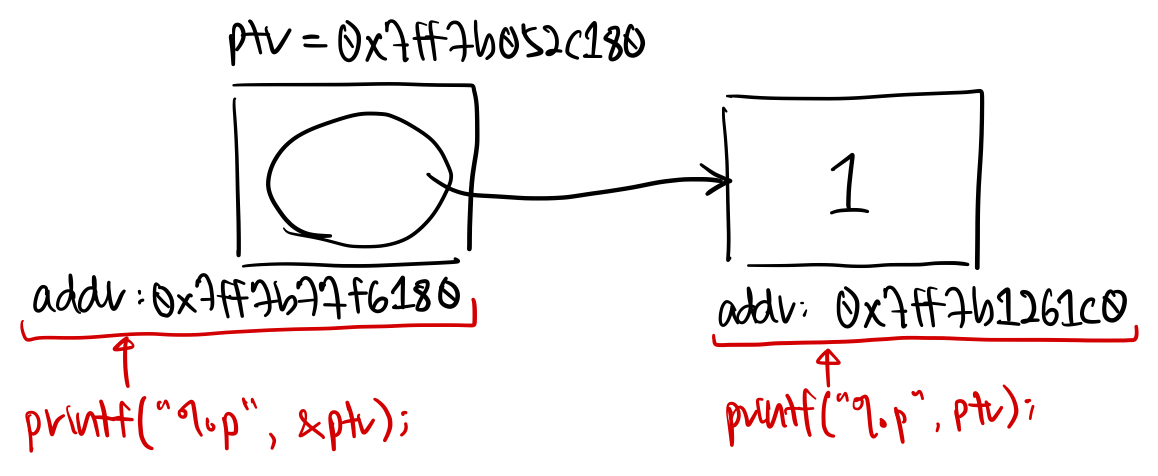
\includegraphics[width=\linewidth]{pointers.jpg}
    % \caption{A boat.}
    % \label{fig:boat1}
\end{figure}

\textbf{Dereferencing} a pointer variable refers to the act of accessing or manipulating a value located at a memory address pointed to by a pointer.
This is done also by adding the asterisk \verb|*| before the pointer variable's name.
Not to be mistaken with declaring pointer variables, this typically happens when trying to access the value located in the memory address being pointed to.
We have seen this in an earlier example with the following line:

\begin{minted}{c}
printf("%d\n", *ptr);
\end{minted}

% concept of pointer, dereferencing
Here's another example:

\begin{minted}[linenos]{c}
int a = 1;
int b[2]; // array of size 2

int *ptr; // pointer to int
ptr = &a; // ptr now points to a
*ptr = 2; // dereference ptr, a is now 2
ptr = &b[1]; // ptr now points to b[1]
\end{minted}

We can also use pointers to point to memory locations in an array.
As seen in these two lines, we initialize \verb|ptr| to point to \verb|a|.
Hence, printing out the value of \verb|ptr| would give the memory address of \verb|a|, while printing that of \verb|*ptr| will render the value of \verb|a| itself, that being 1.


\begin{exercise} \label{pointers1} 
Understanding pointers. \\
State the output of the following code.
Assume memory addresses of variables \verb|m| is \verb|0x3333|,  \verb|n| is \verb|0x5555|, and \verb|p| is \verb|0x2222|.
\begin{minted}[linenos]{c}
int m, *n, **p;

m = 19;
n = &m;
p = &n;

printf("%d / %p\n", m, &m);
printf("%p / %p / %d\n", n, &n, %n);
printf("%p / %p / %p\n", p, &p, %p);

*n = 8;
printf("%d / %p\n", m, n);
\end{minted}
\end{exercise}

\section{Arrays and Pointers}
array decay, pointer arithmetic, using pointers in functions

\begin{minted}[linenos]{c}
/* Note C only has pass by value. 
We use pointers in args to mitigate this. 
Pointer values (addresses) are copied, so we can dereference 
to access underlying value */
void swap(int *x , int *y) {
    int temp;
    temp = *x;
    *x = *y;
    *y = temp;
}

long add_all(long len, int* arr) {
    long res = 0;
    for (int i = 0; i < len; i++) {
        res = res + *(ptr + i);
    }
}

int main() {
    int arr[] = {9, 8, 6, 4, 2};
    long len = 5;

    printf("%d, %d", arr[2], arr[3]);
    swap(arr[2], arr[3]);
    printf("%d, %d", arr[2], arr[3]);

    add_all(len, arr)

    return 0;
}
\end{minted}

\section{Strings}

There is no primitive string data type in C; strings in C are essentially an array of characters with a \verb|NUL| character (\verb|'\0'|) at the end.
You may declare a C string as a \verb|char| array, or a \verb|char| pointer to it, like as follows:

% it's a char array with a NUL at the end!!!

\begin{minted}[linenos]{c}
// Both define strings with the value "ice-cream" 
char[10] str1 = "ice-cream";
char* str2 = "ice-cream";
\end{minted}

Here, the first definition creates a 10-character array \verb|str1| containing the characters 
\verb|'i'|, \verb|'c'|, \verb|'e'|, \verb|'-'|, \verb|'c'|, \verb|'r'|, \verb|'e'|, \verb|'a'|, \verb|'m'| and \verb|'\0'|.
When defining a character array to contain a string, you must ensure that it is large enough to contain each character in the string, as well as the \verb|NUL| (\verb|'\0'|).

\begin{minted}{c}
// str1 can also be declared as follows:
char[] str1 = {'i', 'c', 'e', '-', 'c', 'r', 'e', 'a', 'm', '\0'};
\end{minted}

The second definition creates a pointer variable \verb|str2| which points to the string \verb|"ice-cream"| somewhere in memory.
Here, there need not be a predefined size as to how big the array should be; the size is calculated automatically based on how many characters are included in the string.

\begin{minted}[linenos]{c}
// You can use scanf to store string values.
// No "&" before "word"; "word" acts as a pointer to a string value
scanf("%s", word); 
\end{minted}

\warningbox{
    \begin{typewriter}scanf\end{typewriter} will read characters until a space, tab, newline or end-of-file (EOF) indicator is encountered.
    To prevent crashes due to reading more characters than the available space allocated (e.g., entered string of length 10 to occupy a char array of size 9),
    you can specify the field width in the conversion specifier (e.g., \begin{typewriter}\%9s\end{typewriter}
    - reads 19 characters maximum and saves last character for \begin{typewriter}NUL\end{typewriter} (\begin{typewriter}\textbackslash0\end{typewriter})).
}


\section{Structs}

\textbf{Structures}, or \textit{structs}, are a collection of related variables under one name.
In contrast to arrays which are a collection of variables of the same type (e.g., all \verb|int|s), struct variables can be of different types.
Consider the following struct definition below:

\begin{minted}{c}
struct pt
{
    int x;
    int y;
}; // remember to add the semicolon after struct definition
\end{minted}

Here, we use the keyword \verb|struct| to define a struct, followed by \verb|pt| as its identifier name.
The members of the struct refer to the variables declared within the braces of the struct definition (in this case, they are integer variables \verb|x| and \verb|y|).

Structs act as new data types that can be used to define variables.
The listing below demonstrates how to define a variable of the struct \verb|pt| data type, followed by how to access the struct's members.

\begin{minted}{c}
// we access via name.member
struct pt p;
p.x  = 1;
p.y = 2;
\end{minted}

Since structs act as data types usable for defining variables, we can also use them in function definitions, as well as declare pointers to values of the struct's data type.
Using pointers to structs can be useful, especially with creating some data structures like linked lists.

\begin{minted}[linenos]{c}
/* functions and struct arguments */
struct pt scale_point(struct pt p1, int scale)
{
    p1.x *= scale;
    p1.y *= scale;
    return p1;
}

// we can also use ptrs to structs
void do_nothing(struct pt *p)
{
    int x = p->x; // shorthand for (*p).x
}
\end{minted}

By now, you may have caught on that you require the keyword \verb|struct| to be used whenever you try to reference the declared struct data type.
The keyword \verb|typedef| can be used to reduce the need for necessitating the \verb|struct| keyword to be used each time it is referenced.
\verb|typedef| provides a synonym mechanism for previously defined data types.

To declare the earlier example using \verb|typedef|, we add on to the normal struct definition by adding \verb|typedef| before the \verb|struct| keyword, and a special name right after the struct's braces.
Here, we redeclared \verb|struct pt| to be synonymous to \verb|Pt|.
Hence, we can declare a \verb|struct pt| variable simply by calling \verb|Pt| instead.

\begin{minted}[linenos]{c}
typedef struct pt
{
    int x;
    int y;
} Pt;

Pt p; // Ah.. much shorter, much better. :)

p.x  = 1;
p.y = 2;
\end{minted}

Here is a summary of the code illustrated in this section.

\begin{minted}[linenos]{c}
/* defining and initializing structs */
struct pt
{
    int x;
    int y;
};

// we access via name.member
struct pt p;
p.x  = 1;
p.y = 2;

/* functions and struct arguments */
struct pt scale_point(struct pt p1, int scale)
{
    p1.x *= scale;
    p1.y *= scale;
    return p1;
}
// we can also use ptrs to structs
void do_nothing(struct pt *p)
{
    int x = p->x; // shorthand for (*p).x
}

/* to avoid those cumbersome struct keywords */
typedef struct xd {
    int owo;
    int uwu;
} xd;
// consider cutting into struct + typedef indiv

int main() {
    xd arr[100]; // array of 100 xds
}
\end{minted}